\documentclass[11pt]{report}

\usepackage{epsf,amsmath,amsfonts}
\usepackage{graphicx}
\usepackage{color}

\setlength{\textwidth}{6.5in}
\setlength{\oddsidemargin}{0in}
\setlength{\evensidemargin}{0in}
\setlength{\textheight}{8.5in}
\setlength{\topmargin}{0in}

\begin{document}

\title{
Requirements and Design\\
Ocean Analysis Core (OAC)}
\author{MPAS Development Team}

\maketitle
\tableofcontents

%-----------------------------------------------------------------------

\chapter{Summary}

Now that MPAS-O is well developed and tested, it is time to add an extensible and forward-looking analysis functionality to the MPAS-Ocean model.  Much of the analysis (diagnostics) developed to date has used a post-processing work-flow with Matlab or Python.  These tools have been useful to meet short-term requirements, but they do not scale well to high resolution, and are typically created individually by each developer without coordination, review, or commits to the repository.

This design document lays out a new ocean analysis functionality, where analysis modules such as global means, zonal means, MOC, Lagrangian particles, etc, may be called at run time from the ocean core or as a post-processing step using the Ocean Analysis Core (OAC).  Advantage are that all MPAS grid variables and operators are available within the analysis modules; analysis routines will fall under the same review process and revision control as other code; and once developed, analysis routines are available to all users.

This document only deals with the overall design of the analysis modules and analysis core, not the details of any new diagnostics added within this new framework.  The global diagnostics, which already exist, will be used to test this new design. 

%-----------------------------------------------------------------------

\chapter{Requirements}

Color key: {\color{green} green has been reviewed or is straightforward}, {\color{red} red needs further review}.

\section{Overall organization}
\subsection{{\color{green} Requirement:} OAC may be executed in-situ (i.e. during runtime) or as a post-processing step.}

\subsection{{\color{green} Requirement:} When executed in-situ, OAC may be conducted on the same processors as used for the forward model or on a separate set of processor. In that, OAC can execute in single-program, multiple-data (SPMD) or multiple-program, multiple-data (MPMD) mode. \label{requirement: modes}}
Stated otherwise, OAC can be executed ``in-line'' (OAC-SPMD) with the forward model and can be called (when needed) as a part of the time-stepping sequence. Alternatively, OAC can be executed with a separate MPI communicator (OAC-MPMD) and, thus, executed on dedicated processors that are different from those used for the forward model integration.

This requirement will not be part of the initial implementation due to its complexity, but should not be built out of the design.

\subsection{{\color{green} Requirement:} Analysis algorithms are unaware of the executing environment.}
Below the OAC driver level, the analysis methods are incognizant of whether the operating environment is OAC-SPMD, OAC-MPMD or OAC-PP.

\subsection{{\color{green} Requirement:} Analysis computations will be organized in groups of related computations, controlled in a coherent manner.}
Each {\it analysis member} will have an identical template structure for namelists and code, including flags, timers, init and finalize routines, and the top-level subroutine interface. A template will be included to guide developers for the creation of a new OAC analysis member.

\subsection{{\color{red} Requirement:} Each OAC analysis member is compiled into its own library.}
In order to promote modularity and reuse of object code, each analysis member is to be compiled into its own library that are loaded, along with a driver, to produce OAC.

Like the requirement \ref{requirement: modes}, this requirement will not be part of the initial implementation, but should not be built out of the design.

\newpage
\section{Input data and files}

\subsection{{\color{green} Requirement:} All analysis variables are intent(in).}
No data is returned to the forward model.  The only output is by writing analysis member data to disk.

\subsection{{\color{red} Requirement:} When viewed from the OAC driver and from each OAC analysis member, intent(in) variables are ``state'' and ''analysisInput'' derived data types. Our aspiration is that ``analysisInput'' is empty.}
The modularity, extensibility and repurposing of OAC analysis member will be optimized by limiting the scope of intent(in). The optimal realization of this aspiration would be that OAC operates with only knowledge of the MPAS-O prognostic variables. The requirement here acknowledges our imperfect knowledge of the feasibility of this aspiration.

The upside benefit of this approach is that by minimizing the data flow between MPAS-O and OAC, we reduce risks related to communication bottlenecks and redundant memory allocations. Furthermore, if intent(in) is entirely contained within state, OAC will be able to execute with access of output files or restart files. The downside risk that relatively expensive computations might have to be recomputed. Furthermore, it may turn out that analysis members will require accumulated and/or time-averaged fields from MPAS-O. Thus, we allow for the creation of a new derived data type, {\bf analysisInput}, where auxiliary data can be transferred to OAC. We set a very high bar of adding variable arrays into {\bf analysisInput}.

\newpage
\section{Analysis Member Output}
\subsection{{\color{red} Requirement:} output file format}
All analysis members will write netCDF files along with the derived meta data from the registry in manner identical the current paradigm with MPAS-O. Additional types of output format are permitted, but auxiliary workflow items should be constructed on top of the self-describing netCDF output files. This includes hooks into Paraview, UV-CDAT and similar.

\newpage
\section{Code structure}
\subsection{{\color{green} Requirement:} Redundant computations are computed with identical software.\label{requirement: redundant code}}
This means that computation of diagnostic variables like kinetic energy would not appear in both the ocean and analysis cores. This implementation of this requirement is to force a more modular computation of auxiliary (i.e. diagnostic) data structures.

\subsection{{\color{red} Requirement:} Each OAC-AM (OAC-Analysis Member) resides within a single module.}

\subsection{{\color{red} Requirement:} Analysis Member A can not contain the ``use'' of Analysis Member B.}
If compelling reasons for ``cross talk'' between different analysis members are presented, then the two analysis members should be merged into a single analysis member.

\subsection{{\color{red} Requirement:} All MPAS-O computations that are not needed to move the model forward in time are to occur within the analysis core.}
This is similar to requirement \ref{requirement: redundant code}, but specifies that all diagnostics, computation of means and variability, etc. must be in the analysis core.  

One question is: kinetic energy, vorticity, density, pressure, etc. appear in the momentum equation and are needed to 'move the model forward'.  Where should they go?  i.e., is the converse true: All MPAS-O computations that {\bf are} needed to move the model forward in time are to occur within the {\bf ocean} core?

Todd: KE, vorticity, etc are required to move the model forward in time, so these are computed in MPAS-O. These same variable might be recomputed in OAC.

\subsection{{\color{green} Requirement:} All namelist flags and variables only appear once among all the registry files.}
A newly added analysis flag or variable should only be added to a single registry file.  This prevents errors of requiring duplicate entries in the ocean and analysis registry files.

\subsection{{\color{red} Requirement:} Analysis core does not use subroutines from ocean core.}
In the hierarchy of subroutines, the ocean time-stepping routine will call analysis subroutines.  If analysis core routines can call ocean core routines as well, there is the possibility of recursive 'use' statements in the modules.

One possible exception to this is an analysis group that computes tendency terms.  In order for computations to only appear once and only pass prognostic variables into the analysis core, the analysis routine must call tendency routines in the ocean core.


%% \section{{\color{green} Requirement:} Analysis routines may be applied during run-time or post-processing}
%% Date last modified: 2013/10/15 \\
%% Contributors: Mark Petersen \\

%% Run-Time or post-processing work-flows will call the same subroutines.  Output must be identical for both processes.

%% \section{{\color{green} Requirement:} Post-processing must work on both output and restart files}
%% Date last modified: 2013/10/15 \\
%% Contributors: Mark Petersen \\

%% This requirement is up for discussion.  Should the analysis core be required to function on restart files?  One issue is that some variables, particularly time means and time variances, are missing from restart files.  If applied to restart files, those arrays would simply fill in with zeros.

%% \section{{\color{green} Requirement:} Each analysis group will have its own flags, timers, and output files}
%% Date last modified: 2013/10/15 \\
%% Contributors: Mark Petersen \\

%% An analysis group is a group of statistics that are computed at the same time.  Examples of analysis groups are:
%% \begin{itemize}
%% \item global statistics
%% \item MOC
%% \item zonal averages
%% \end{itemize}
%% For simplicity of organization, flags, timers, and output files will use this same grouping.

%% \section{{\color{green} Requirement:} Each analysis group may have its own output format}
%% Date last modified: 2013/10/15 \\
%% Contributors: Mark Petersen \\

%% Some analysis groups, like global diagnostics, may use text files with one line per output time.  Other analysis groups may produce netcdf files or other formats.  Output from analysis modules should not be placed in the run-time output*.nc files.


%-----------------------------------------------------------------------


\chapter{Design and Implementation}

\section{Overview}
The conceptual layout of each OAC-AM is portrayed in Figure \ref{OAC-AM}. Each OAC-AM will have four points of entry.

\begin{figure}[p]
\center{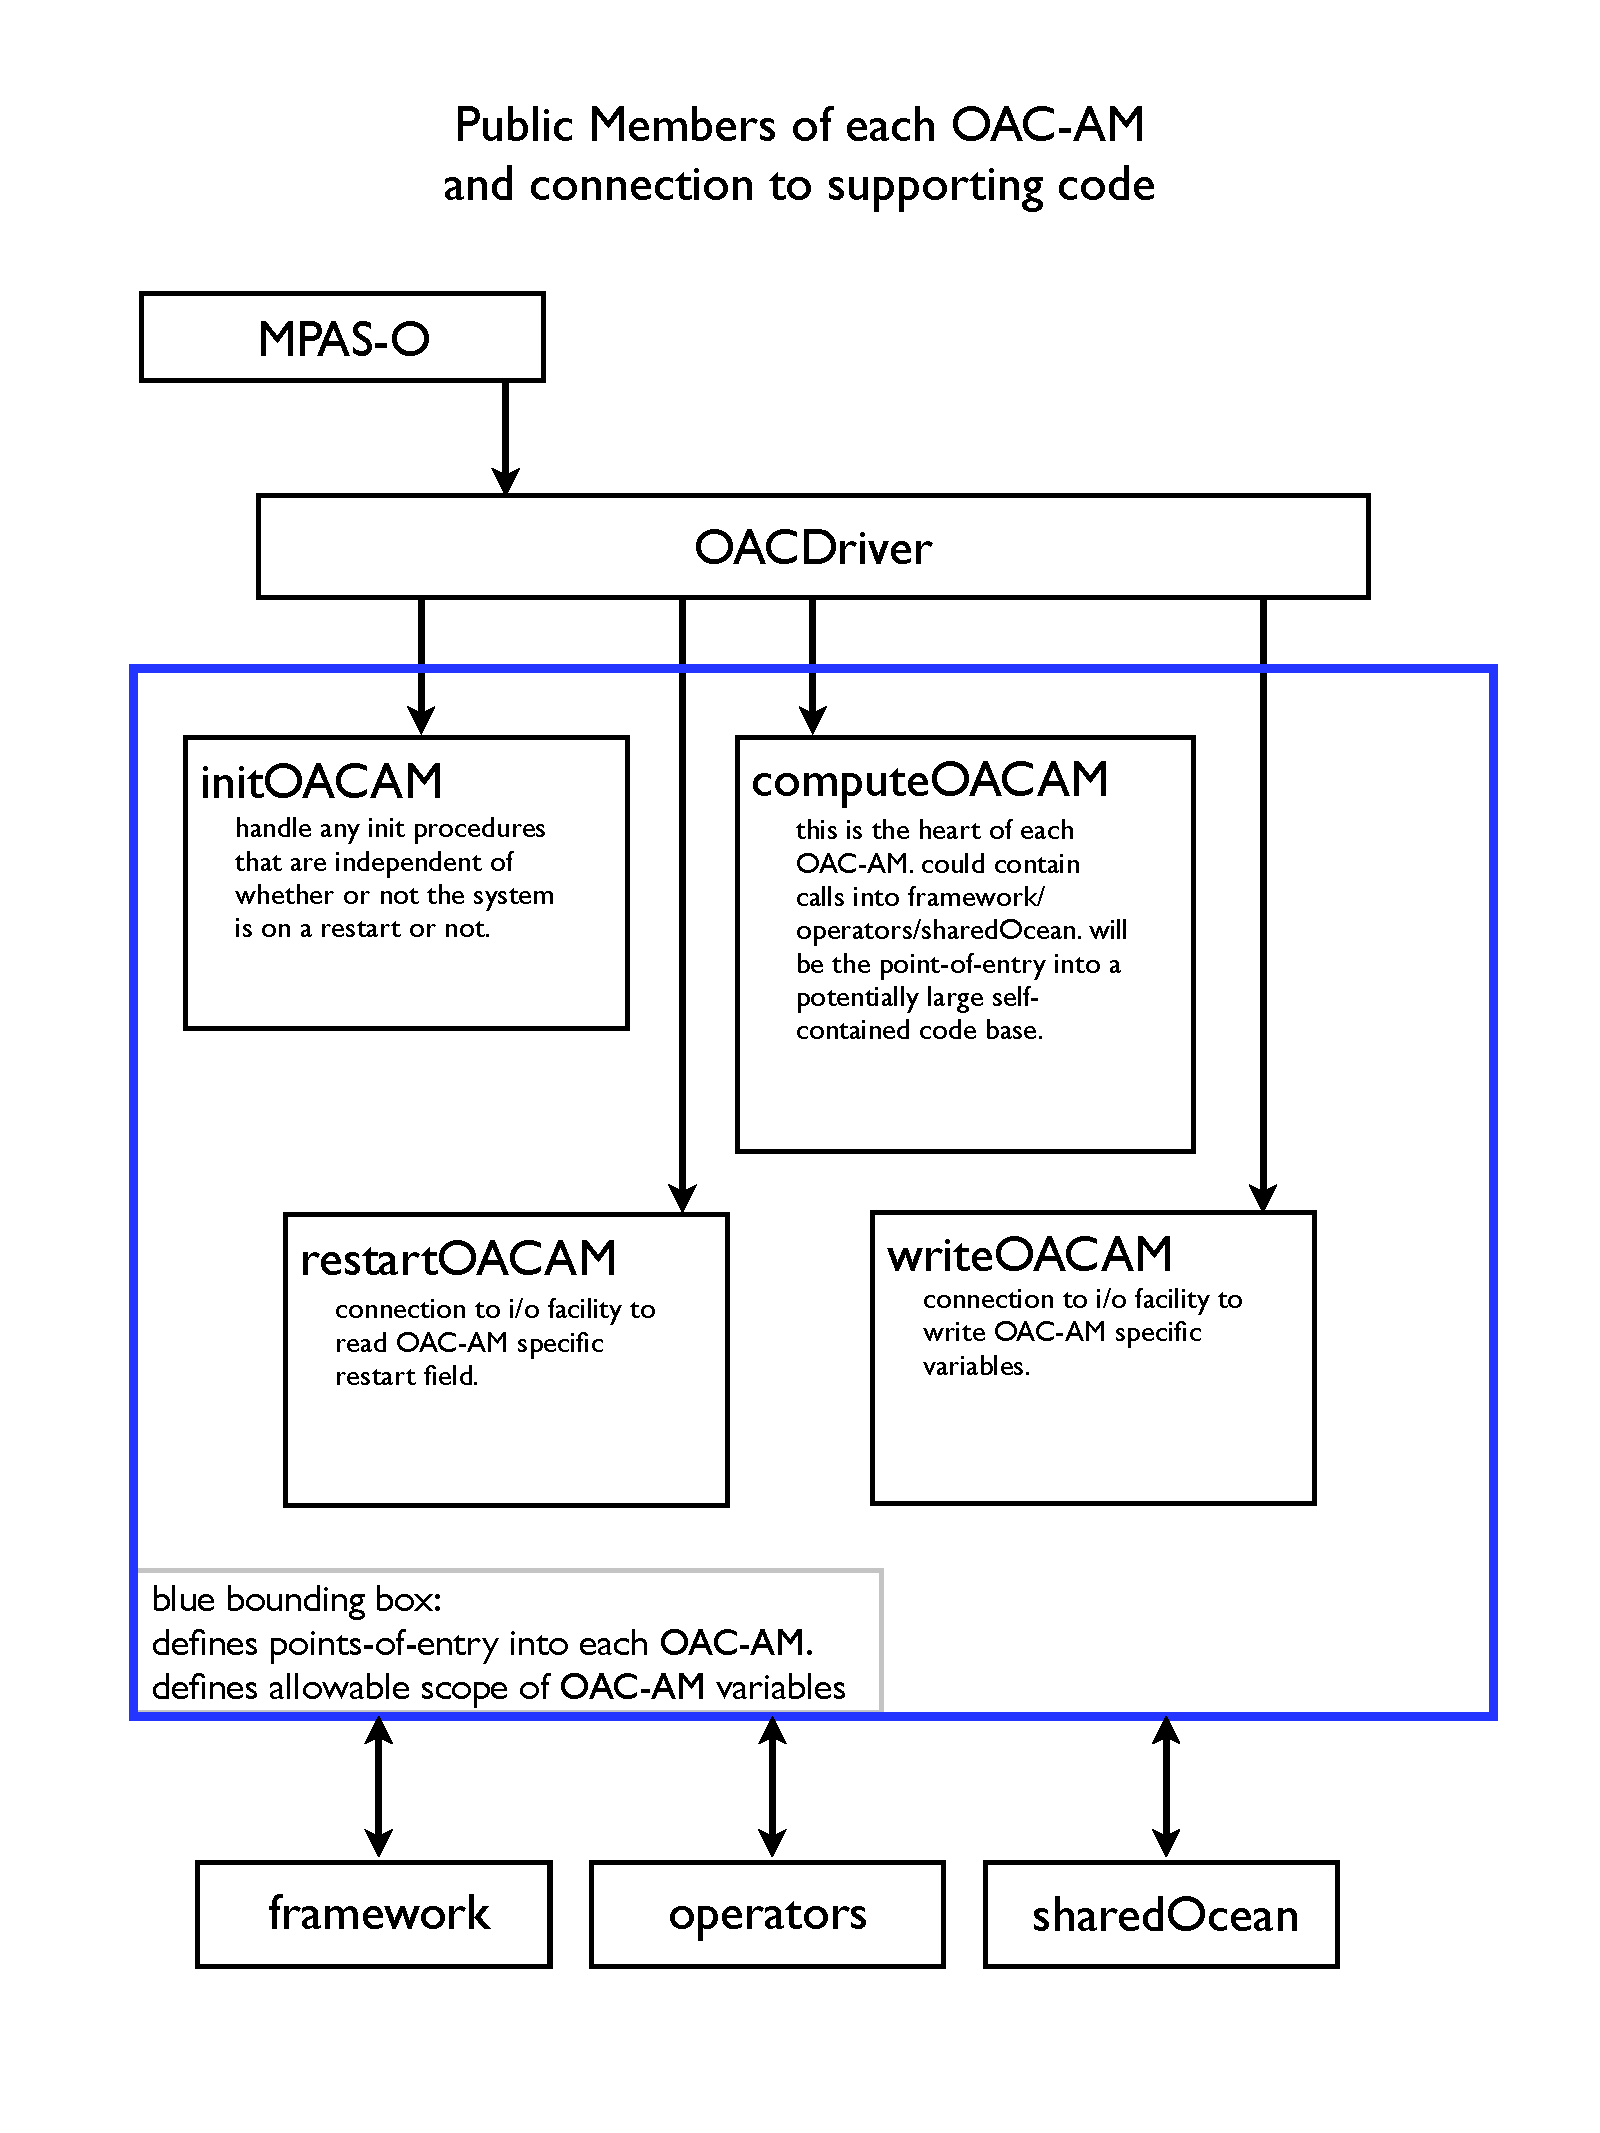
\includegraphics[width=12.0cm]{./figures/OAC-AM.pdf}} \\
\caption{Diagram outlining the calls into each analysis member.}
\label{OAC-AM}
\end{figure}

\section{Definition OAC-AM points-of-entry}

\subsection{initOACAM}

\subsection{restartOACAM}

\subsection{computeOACAM}

\subsection{writeOACAM}


\section{Definition of minimum set of OAC-AM namelist record}
Each OAC-AM will have a standardized, minimum set of config namelist entries. This list can be augmented for each OAC-AM.

\subsection{executeAM}

(maybe put all of this into a .tex table)



%% \section{Implementation: Analysis routines may be applied during run-time or post-processing}
%% Date last modified: 2013/10/15 \\
%% Contributors: Mark Petersen \\

%% The directory structure will be as follows:
%% \begin{itemize}
%% \item MPAS/src/
%% \begin{itemize}
%% \item core\_ocean
%% \begin{itemize}
%% \item mpas\_ocn\_mpas\_core.F, etc
%% \end{itemize}
%% \item core\_ocean\_analysis
%% \begin{itemize}
%% \item mpas\_ocn\_analysis\_mpas\_core.F
%% \item mpas\_ocn\_analysis\_global\_stats.F
%% \item mpas\_ocn\_analysis\_moc.F
%% \item mpas\_ocn\_analysis\_zonal\_avg.F, etc
%% \end{itemize}
%% \end{itemize}
%% \end{itemize}

%% The analysis core may be compiled using\\
%% make {\it target} CORE=ocean\_analysis

%% \newpage
%% \section{Implementation: Each analysis group will have its own timer and output files}
%% Date last modified: 2013/10/15 \\
%% Contributors: Mark Petersen \\

%% The new namelists for the ocean core will be:
%% \begin{verbatim}
%% &analysis
%%    config_write_analysis_on_startup = .true.
%%    config_write_global_stats = .true.
%%    config_global_stats_interval = "0001_00:00:00"
%%    config_write_moc = .true.
%%    config_moc_interval = "0001_00:00:00"
%%    config_write_zonal_avg = .true.
%%    config_zonal_avg_interval = "0001_00:00:00"
%%    etc
%% /
%% \end{verbatim}
%% The \verb|stats| flags will be removed from the io namelist.  One option for the interval flags will be 
%% \begin{verbatim}
%%    config_global_stats_interval = "output_interval"
%% \end{verbatim}
%% which sets it to the save value as \verb|config_output_interval|.

%% The new namelists for the ocean analysis core will be:
%% \begin{verbatim}
%% &io
%%    config_filename = "output.0000-01-01_00.00.00.nc"
%%    config_filename_list = "filename_list"
%%    config_first_record = 1
%%    config_record_interval = 1
%%    config_last_record = 1000
%%    config_pio_num_iotasks = 0
%%    config_pio_stride = 1
%% /
%% &analysis
%%    config_write_global_stats = .true.
%%    config_write_moc = .true.
%%    config_write_zonal_avg = .true.
%%    etc
%% /
%% \end{verbatim}

%% If \verb|config_filename = "file"| then the analysis core proceeds through the list of filenames provided in 
%% \verb|config_filename_list|.
%% %-----------------------------------------------------------------------

%% \chapter{Testing}

%% \section{Testing: Analysis routines may be applied during run-time or post-processing}
%% Date last modified: 2013/10/15 \\
%% Contributors: Mark Petersen \\

%% After completion, a global simulation will be conducted with run-time analysis tools on.  Global diagnostics output will be compared between run-time, post-processed analysis core data, and global statistics from the current develop branch.  All three should match bit-for-bit on the same number of processors.  When processor counts vary, global statistics may not match in last digits due to order of operations.



%-----------------------------------------------------------------------

\end{document}
